\documentclass[10pt]{article}
\usepackage[utf8]{inputenc}
\usepackage[french]{babel}
% Style commun aux CV FR et EN (reproduit le modèle visuel d'origine)
\usepackage[T1]{fontenc}
\usepackage{lmodern}
\usepackage{geometry}
\usepackage{graphicx}
\usepackage{xcolor}
\usepackage{tikz}
\usepackage{tabularx}
\usepackage[letterspace=50]{microtype}
\usepackage[hidelinks]{hyperref}

\geometry{a4paper,left=0.87cm,right=0.87cm,top=0.5cm,bottom=0.4cm}
\pagestyle{empty}
\setlength{\parindent}{0pt}
\setlength{\parskip}{0pt}

\definecolor{mainblue}{HTML}{1A5DAB}
\definecolor{darktext}{HTML}{1A1A1A}
\definecolor{muted}{HTML}{6B6B6B}

\newcommand{\bluelink}[2]{\href{#1}{\textcolor{mainblue}{\textbf{#2}}}}
\newcommand{\sep}{\quad|\quad}

% Titre de section : bleu, gras, majuscules, filet fin bleu
\newcommand{\cvsection}[1]{%
  \par\vspace{4pt}%
  {\fontsize{10.5}{12}\selectfont\bfseries\color{mainblue}\textls[60]{#1}}\par\vspace{2pt}%
  {\color{mainblue}\hrule height 0.5pt}\par\vspace{2pt}%
}

% Ligne titre (gras) à gauche, info grise à droite
\newcommand{\entry}[2]{%
  \par\noindent\textbf{#1}\hfill{\color{muted}#2}\par
}

% Puce tiret
\newcommand{\dash}[1]{\par\noindent\hangindent=1.4em\hangafter=1 \makebox[1.4em][l]{\,--}#1\par}

\newcommand{\techsep}{\enspace\textbullet\enspace}

% En-tête : photo ronde + nom, sous-titre, coordonnées, liens
\newcommand{\cvheader}[1]{%
  \noindent
  \begin{minipage}[c]{0.215\linewidth}
    \begin{tikzpicture}
      \begin{scope}
        \clip (0,0) circle (1.52cm);
        \node at (0,-0.5) {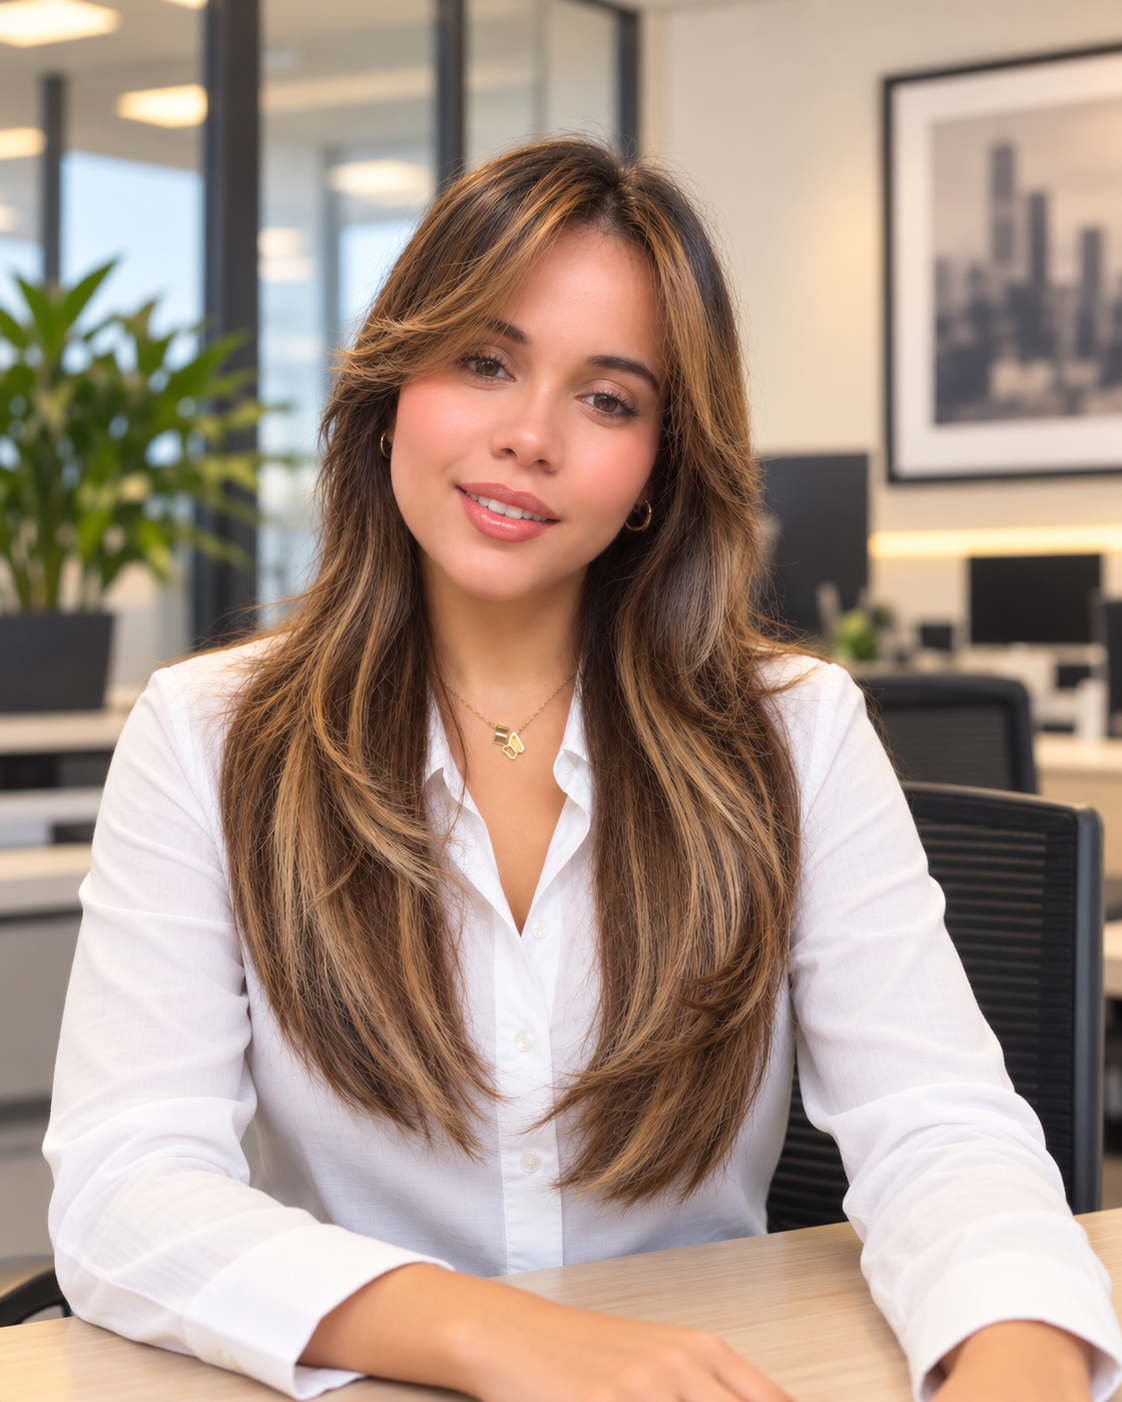
\includegraphics[width=3.3cm]{../public/images/photo.jpg}};
      \end{scope}
      \draw[mainblue,line width=0.5pt] (0,0) circle (1.52cm);
    \end{tikzpicture}
  \end{minipage}\hspace{0.6cm}%
  \begin{minipage}[c]{0.72\linewidth}
    {\fontsize{25}{28}\selectfont\bfseries\textls[35]{MALEK GHABI}}\par\vspace{3pt}
    {\fontsize{12}{14}\selectfont\bfseries\color{mainblue}#1}\par\vspace{4pt}
    {\fontsize{9.5}{12}\selectfont Cluses, France\sep+33 6 04 10 21 56\sep\href{mailto:malekghabi.education@gmail.com}{malekghabi.education@gmail.com}}\par\vspace{3pt}
    {\fontsize{10}{12}\selectfont\bluelink{https://github.com/malekghabi1607}{GitHub}\sep\bluelink{https://www.linkedin.com/in/malek-ghabi-3b3267a9/}{LinkedIn}\sep\bluelink{https://malekghabi.netlify.app}{Portfolio}}
  \end{minipage}\par\vspace{2pt}
}

% Taille du corps de texte (ajustée pour tenir sur une page)
\AtBeginDocument{\fontsize{9.3}{11.1}\selectfont}


\begin{document}
\color{darktext}\fontsize{9.3}{11.1}\selectfont

\cvheader{Développeuse Software \& Data \,|\, Alternante chez NOVOUTILS}

\cvsection{PROFIL}
{\fontsize{9.6}{11.6}\selectfont
Diplômée d'une Licence Informatique à Avignon Université, je poursuis un Master Informatique à l'Université Catholique de Lille, parcours Informatique appliquée et systèmes intelligents, en alternance chez NOVOUTILS\@. Je m'intéresse au développement logiciel, à la data, aux bases de données et à l'intelligence artificielle, avec l'objectif de concevoir des solutions fiables, utiles et adaptées aux besoins métier.\par}

\cvsection{COMPÉTENCES}
\textbf{Langages:} Java, Python, JavaScript, TypeScript, SQL, PHP, C/C++, Bash, HTML5, CSS3\par
\textbf{Back-End \& API:} Spring Boot, FastAPI, Flask, Laravel, REST API, JWT, WebSockets, Swagger/OpenAPI\par
\textbf{Front-End:} React, Vite, Tailwind CSS, Bootstrap, AJAX, Chart.js\par
\textbf{Bases de données:} PostgreSQL, MySQL, SQLite, Supabase, Firebase, conception et migration de données\par
\textbf{Data \& automatisation:} Pandas, NumPy, Scikit-Learn, Excel, Power BI, traitement de fichiers, visualisation de données\par
\textbf{DevOps \& outils:} Git, GitHub, Docker, Docker Compose, GitHub Actions, Linux, Nginx, Postman, VS Code, IntelliJ\par
\textbf{Méthodes:} POO, architecture MVC, UML, Agile/Scrum, tests, documentation technique\par
\textbf{Compétences personnelles:} Autonomie, rigueur, organisation, curiosité, travail en équipe, adaptabilité\par

\cvsection{PROJETS TECHNIQUES}
\entry{Aura Student Life OS}{React\techsep{}Spring Boot\techsep{}PostgreSQL\techsep{}Docker}
Plateforme SaaS full-stack d'organisation de la vie étudiante: finances, objectifs, planning, habitudes, sport et assistant IA.\par
\dash{Architecture full-stack: frontend React/Vite, API REST Spring Boot documentée (Swagger/OpenAPI), PostgreSQL et Docker.}
\dash{Authentification Spring Security/JWT, tableaux de bord interactifs, exports Excel/PDF et assistant IA connecté à l'API.}
\dash{Conception modulaire de plusieurs domaines métier réunis dans un dashboard global d'indicateurs personnels.}
\vspace{1pt}
\entry{Snake IA \textemdash{} Hackathon 24h pour coder}{JavaScript\techsep{}Canvas\techsep{}A*\techsep{}Q-Learning}
Version avancée du jeu Snake développée en 24 h, avec une intelligence artificielle adaptative.\par
\dash{Bête IA évolutive dont le comportement s'adapte au joueur grâce à l'apprentissage par renforcement (Q-Learning).}
\dash{Recherche de chemin optimal avec A* et points intelligents qui fuient le Snake via l'algorithme des Boïds.}
\dash{Coordination de plusieurs algorithmes d'IA en temps réel sans perte de performance, interface fluide en Canvas.}
\vspace{1pt}
\entry{EasyMonitor}{Bash\techsep{}Python\techsep{}Flask\techsep{}SQLite\techsep{}Chart.js}
Outil de supervision système distribué permettant de surveiller plusieurs machines virtuelles via une interface web.\par
\dash{Agent Bash/Python collectant CPU, RAM, disque, réseau et utilisateurs, transmis au serveur Flask via HTTP sécurisé.}
\dash{Stockage SQLite/RRDTool, graphiques temps réel et historiques, alertes automatiques (CPU, mémoire, disque plein).}
\dash{Communication réseau entre deux VM, authentification des agents et optimisation de la fréquence de collecte.}
\vspace{1pt}
\entry{WithYou}{React\techsep{}Laravel\techsep{}Socket.io\techsep{}Supabase}
Plateforme collaborative de visionnage synchronisé en temps réel, développée en équipe de 5 --- MVP en cours de développement.\par
\dash{Lecture vidéo synchronisée (YouTube IFrame API), salons virtuels et chat temps réel via Socket.io et Laravel Reverb.}
\dash{API Laravel avec authentification JWT, gestion des membres et des permissions par rôle, sondages et salons publics.}
\dash{Architecture en 3 services (client React/Vite, API Laravel, service temps réel), déploiement prévu sur Netlify/Render/Railway.}
\vspace{1pt}
\entry{Moteur de Recherche}{Java\techsep{}Indexation\techsep{}TF-IDF}
Moteur de recherche simplifié avec analyse de corpus, indexation et classement par pertinence.\par
\dash{Normalisation du texte (casse, ponctuation, stop-words) et construction d'un index inversé (terme $\rightarrow$ documents).}
\dash{Pondération TF-IDF, similarité cosinus et classement des meilleurs résultats sur des corpus Wikipédia et ouvrages.}
\dash{Deux modes de vocabulaire (complet ou réduit) et API permettant de brancher facilement de nouveaux corpus.}

\cvsection{EXPÉRIENCES PROFESSIONNELLES}
\entry{Apprentie Software \& Data Engineer \textemdash{} NOVOUTILS, Thyez}{Septembre 2026 \textendash{} Présent}
\dash{Refonte d'une architecture de base de données connectée à l'ERP CEGID PMI\@: analyse, structuration et migration.}
\dash{Amélioration d'une solution Power BI de suivi commercial: tableaux de bord, indicateurs et reporting automatisé.}
\dash{Conception d'une application de gestion d'équipements de mesure: contrôle d'accès, journalisation, sauvegarde et notifications.}
\dash{Contribution à la coordination d'un projet logiciel orienté IA, entre besoins métier et spécifications techniques.}
\vspace{1pt}
\entry{Stagiaire Développeuse Full-Stack \textemdash{} CEA Marcoule}{Mai 2026 \textendash{} Août 2026}
\dash{Développement de CADI Web, application interne de modernisation des processus de formation de l'INSTN/CEA.}
\dash{Création d'interfaces React/TypeScript et d'API Python/FastAPI intégrant les outils de traitement existants.}
\dash{Automatisation du traitement de fichiers Excel, Word et CSV avec suivi d'avancement et journalisation.}
\dash{Participation à l'architecture logicielle, aux tests, au débogage et au versionnement avec Git.}

\cvsection{FORMATION}
\entry{Master Informatique \textemdash{} Informatique appliquée et systèmes intelligents}{2026 \textendash{} 2028}
Université Catholique de Lille \textemdash{} alternance chez NOVOUTILS\par\vspace{0.5pt}
\entry{Licence Informatique}{2023 \textendash{} 2026}
Avignon Université, France\par\vspace{0.5pt}
\entry{Bachelor en sciences informatiques}{2025 \textendash{} 2026}
Université de Genève, Suisse \textemdash{} double cursus avec la Licence d'Avignon, première année suivie\par\vspace{0.5pt}
\entry{Baccalauréat Général Scientifique}{2023}
Lycée Jean-Henri Fabre, France\par

\cvsection{LANGUES}
Français: courant\sep{}Anglais: professionnel\sep{}Arabe: courant\sep{}Italien: intermédiaire

\end{document}
